% Options for packages loaded elsewhere
\PassOptionsToPackage{unicode}{hyperref}
\PassOptionsToPackage{hyphens}{url}
\PassOptionsToPackage{dvipsnames,svgnames,x11names}{xcolor}
%
\documentclass[
  a4paper,
  DIV=11,
  numbers=noendperiod]{scrreprt}

\usepackage{amsmath,amssymb}
\usepackage{iftex}
\ifPDFTeX
  \usepackage[T1]{fontenc}
  \usepackage[utf8]{inputenc}
  \usepackage{textcomp} % provide euro and other symbols
\else % if luatex or xetex
  \usepackage{unicode-math}
  \defaultfontfeatures{Scale=MatchLowercase}
  \defaultfontfeatures[\rmfamily]{Ligatures=TeX,Scale=1}
\fi
\usepackage{lmodern}
\ifPDFTeX\else  
    % xetex/luatex font selection
\fi
% Use upquote if available, for straight quotes in verbatim environments
\IfFileExists{upquote.sty}{\usepackage{upquote}}{}
\IfFileExists{microtype.sty}{% use microtype if available
  \usepackage[]{microtype}
  \UseMicrotypeSet[protrusion]{basicmath} % disable protrusion for tt fonts
}{}
\makeatletter
\@ifundefined{KOMAClassName}{% if non-KOMA class
  \IfFileExists{parskip.sty}{%
    \usepackage{parskip}
  }{% else
    \setlength{\parindent}{0pt}
    \setlength{\parskip}{6pt plus 2pt minus 1pt}}
}{% if KOMA class
  \KOMAoptions{parskip=half}}
\makeatother
\usepackage{xcolor}
\setlength{\emergencystretch}{3em} % prevent overfull lines
\setcounter{secnumdepth}{-\maxdimen} % remove section numbering
% Make \paragraph and \subparagraph free-standing
\ifx\paragraph\undefined\else
  \let\oldparagraph\paragraph
  \renewcommand{\paragraph}[1]{\oldparagraph{#1}\mbox{}}
\fi
\ifx\subparagraph\undefined\else
  \let\oldsubparagraph\subparagraph
  \renewcommand{\subparagraph}[1]{\oldsubparagraph{#1}\mbox{}}
\fi

\usepackage{color}
\usepackage{fancyvrb}
\newcommand{\VerbBar}{|}
\newcommand{\VERB}{\Verb[commandchars=\\\{\}]}
\DefineVerbatimEnvironment{Highlighting}{Verbatim}{commandchars=\\\{\}}
% Add ',fontsize=\small' for more characters per line
\usepackage{framed}
\definecolor{shadecolor}{RGB}{241,243,245}
\newenvironment{Shaded}{\begin{snugshade}}{\end{snugshade}}
\newcommand{\AlertTok}[1]{\textcolor[rgb]{0.68,0.00,0.00}{#1}}
\newcommand{\AnnotationTok}[1]{\textcolor[rgb]{0.37,0.37,0.37}{#1}}
\newcommand{\AttributeTok}[1]{\textcolor[rgb]{0.40,0.45,0.13}{#1}}
\newcommand{\BaseNTok}[1]{\textcolor[rgb]{0.68,0.00,0.00}{#1}}
\newcommand{\BuiltInTok}[1]{\textcolor[rgb]{0.00,0.23,0.31}{#1}}
\newcommand{\CharTok}[1]{\textcolor[rgb]{0.13,0.47,0.30}{#1}}
\newcommand{\CommentTok}[1]{\textcolor[rgb]{0.37,0.37,0.37}{#1}}
\newcommand{\CommentVarTok}[1]{\textcolor[rgb]{0.37,0.37,0.37}{\textit{#1}}}
\newcommand{\ConstantTok}[1]{\textcolor[rgb]{0.56,0.35,0.01}{#1}}
\newcommand{\ControlFlowTok}[1]{\textcolor[rgb]{0.00,0.23,0.31}{#1}}
\newcommand{\DataTypeTok}[1]{\textcolor[rgb]{0.68,0.00,0.00}{#1}}
\newcommand{\DecValTok}[1]{\textcolor[rgb]{0.68,0.00,0.00}{#1}}
\newcommand{\DocumentationTok}[1]{\textcolor[rgb]{0.37,0.37,0.37}{\textit{#1}}}
\newcommand{\ErrorTok}[1]{\textcolor[rgb]{0.68,0.00,0.00}{#1}}
\newcommand{\ExtensionTok}[1]{\textcolor[rgb]{0.00,0.23,0.31}{#1}}
\newcommand{\FloatTok}[1]{\textcolor[rgb]{0.68,0.00,0.00}{#1}}
\newcommand{\FunctionTok}[1]{\textcolor[rgb]{0.28,0.35,0.67}{#1}}
\newcommand{\ImportTok}[1]{\textcolor[rgb]{0.00,0.46,0.62}{#1}}
\newcommand{\InformationTok}[1]{\textcolor[rgb]{0.37,0.37,0.37}{#1}}
\newcommand{\KeywordTok}[1]{\textcolor[rgb]{0.00,0.23,0.31}{#1}}
\newcommand{\NormalTok}[1]{\textcolor[rgb]{0.00,0.23,0.31}{#1}}
\newcommand{\OperatorTok}[1]{\textcolor[rgb]{0.37,0.37,0.37}{#1}}
\newcommand{\OtherTok}[1]{\textcolor[rgb]{0.00,0.23,0.31}{#1}}
\newcommand{\PreprocessorTok}[1]{\textcolor[rgb]{0.68,0.00,0.00}{#1}}
\newcommand{\RegionMarkerTok}[1]{\textcolor[rgb]{0.00,0.23,0.31}{#1}}
\newcommand{\SpecialCharTok}[1]{\textcolor[rgb]{0.37,0.37,0.37}{#1}}
\newcommand{\SpecialStringTok}[1]{\textcolor[rgb]{0.13,0.47,0.30}{#1}}
\newcommand{\StringTok}[1]{\textcolor[rgb]{0.13,0.47,0.30}{#1}}
\newcommand{\VariableTok}[1]{\textcolor[rgb]{0.07,0.07,0.07}{#1}}
\newcommand{\VerbatimStringTok}[1]{\textcolor[rgb]{0.13,0.47,0.30}{#1}}
\newcommand{\WarningTok}[1]{\textcolor[rgb]{0.37,0.37,0.37}{\textit{#1}}}

\providecommand{\tightlist}{%
  \setlength{\itemsep}{0pt}\setlength{\parskip}{0pt}}\usepackage{longtable,booktabs,array}
\usepackage{calc} % for calculating minipage widths
% Correct order of tables after \paragraph or \subparagraph
\usepackage{etoolbox}
\makeatletter
\patchcmd\longtable{\par}{\if@noskipsec\mbox{}\fi\par}{}{}
\makeatother
% Allow footnotes in longtable head/foot
\IfFileExists{footnotehyper.sty}{\usepackage{footnotehyper}}{\usepackage{footnote}}
\makesavenoteenv{longtable}
\usepackage{graphicx}
\makeatletter
\def\maxwidth{\ifdim\Gin@nat@width>\linewidth\linewidth\else\Gin@nat@width\fi}
\def\maxheight{\ifdim\Gin@nat@height>\textheight\textheight\else\Gin@nat@height\fi}
\makeatother
% Scale images if necessary, so that they will not overflow the page
% margins by default, and it is still possible to overwrite the defaults
% using explicit options in \includegraphics[width, height, ...]{}
\setkeys{Gin}{width=\maxwidth,height=\maxheight,keepaspectratio}
% Set default figure placement to htbp
\makeatletter
\def\fps@figure{htbp}
\makeatother
\newlength{\cslhangindent}
\setlength{\cslhangindent}{1.5em}
\newlength{\csllabelwidth}
\setlength{\csllabelwidth}{3em}
\newlength{\cslentryspacingunit} % times entry-spacing
\setlength{\cslentryspacingunit}{\parskip}
\newenvironment{CSLReferences}[2] % #1 hanging-ident, #2 entry spacing
 {% don't indent paragraphs
  \setlength{\parindent}{0pt}
  % turn on hanging indent if param 1 is 1
  \ifodd #1
  \let\oldpar\par
  \def\par{\hangindent=\cslhangindent\oldpar}
  \fi
  % set entry spacing
  \setlength{\parskip}{#2\cslentryspacingunit}
 }%
 {}
\usepackage{calc}
\newcommand{\CSLBlock}[1]{#1\hfill\break}
\newcommand{\CSLLeftMargin}[1]{\parbox[t]{\csllabelwidth}{#1}}
\newcommand{\CSLRightInline}[1]{\parbox[t]{\linewidth - \csllabelwidth}{#1}\break}
\newcommand{\CSLIndent}[1]{\hspace{\cslhangindent}#1}

\usepackage{float}
\usepackage{tabularray}
\usepackage[normalem]{ulem}
\usepackage{graphicx}
\UseTblrLibrary{booktabs}
\UseTblrLibrary{siunitx}
\NewTableCommand{\tinytableDefineColor}[3]{\definecolor{#1}{#2}{#3}}
\newcommand{\tinytableTabularrayUnderline}[1]{\underline{#1}}
\newcommand{\tinytableTabularrayStrikeout}[1]{\sout{#1}}
\KOMAoption{captions}{tableheading}
\makeatletter
\makeatother
\makeatletter
\makeatother
\makeatletter
\@ifpackageloaded{caption}{}{\usepackage{caption}}
\AtBeginDocument{%
\ifdefined\contentsname
  \renewcommand*\contentsname{Table of contents}
\else
  \newcommand\contentsname{Table of contents}
\fi
\ifdefined\listfigurename
  \renewcommand*\listfigurename{List of Figures}
\else
  \newcommand\listfigurename{List of Figures}
\fi
\ifdefined\listtablename
  \renewcommand*\listtablename{List of Tables}
\else
  \newcommand\listtablename{List of Tables}
\fi
\ifdefined\figurename
  \renewcommand*\figurename{Figure}
\else
  \newcommand\figurename{Figure}
\fi
\ifdefined\tablename
  \renewcommand*\tablename{Table}
\else
  \newcommand\tablename{Table}
\fi
}
\@ifpackageloaded{float}{}{\usepackage{float}}
\floatstyle{ruled}
\@ifundefined{c@chapter}{\newfloat{codelisting}{h}{lop}}{\newfloat{codelisting}{h}{lop}[chapter]}
\floatname{codelisting}{Listing}
\newcommand*\listoflistings{\listof{codelisting}{List of Listings}}
\makeatother
\makeatletter
\@ifpackageloaded{caption}{}{\usepackage{caption}}
\@ifpackageloaded{subcaption}{}{\usepackage{subcaption}}
\makeatother
\makeatletter
\@ifpackageloaded{tcolorbox}{}{\usepackage[skins,breakable]{tcolorbox}}
\makeatother
\makeatletter
\@ifundefined{shadecolor}{\definecolor{shadecolor}{rgb}{.97, .97, .97}}
\makeatother
\makeatletter
\makeatother
\makeatletter
\makeatother
\ifLuaTeX
  \usepackage{selnolig}  % disable illegal ligatures
\fi
\IfFileExists{bookmark.sty}{\usepackage{bookmark}}{\usepackage{hyperref}}
\IfFileExists{xurl.sty}{\usepackage{xurl}}{} % add URL line breaks if available
\urlstyle{same} % disable monospaced font for URLs
\hypersetup{
  pdftitle={PPML HDFE in R: a short workshop},
  pdfauthor={Krisna Gupta},
  colorlinks=true,
  linkcolor={blue},
  filecolor={Maroon},
  citecolor={Blue},
  urlcolor={Blue},
  pdfcreator={LaTeX via pandoc}}

\title{PPML HDFE in R: a short workshop}
\author{Krisna Gupta}
\date{May 18, 2024}

\begin{document}
\maketitle
\begin{abstract}
This page is dedicated to teach students on running the gravity model in
R. We uses dataset from CEPII, specifically BACI and the gravity
dataset. We run in R and RStudio IDE, and we rely on ppml from the
gravity package when demonstrating PPML. We try to replicate Silva and
Tenreyro (2006), an excellent paper for an introduction to the log
gravity model and PPML.
\end{abstract}
\ifdefined\Shaded\renewenvironment{Shaded}{\begin{tcolorbox}[frame hidden, sharp corners, enhanced, borderline west={3pt}{0pt}{shadecolor}, breakable, interior hidden, boxrule=0pt]}{\end{tcolorbox}}\fi

\hypertarget{sec-introduction}{%
\section{Introduction}\label{sec-introduction}}

The gravity model is probably the most popular model in international
trade. Many uses them. It is very intuitive, great predictive power, and
most importantly, tweakable (Yotov 2022). But the even most important is
that UI students love them. If you're doing trade for your thesis, then
you probably going to use the gravity model as your backbone.

This guide is my attempt to help you learn gravity model much easier.
The most important part is probably the data and the model itself. What
is the minimum things you need in the gravity model, how to arrange the
database, run them, and interpret them. You must familiarize yourself
with the data and its wrangling (80\% of your coding) as well as the
main gravity specification to date. I encourage students to pay careful
attention to Yotov (2022) as it hosts the recent development in the
gravity model, a must read if you're planning to utilize gravity model.

I use R here because I use R much more than Stata these days. However,
the two language aren't very different. You can do the same thing on
both, but you may need to google a bit. It's okay to use google a lot. I
did as well even right now. Oh yeah I also informed you guys know R
already so I won't go into too much basic stuff.

Next is the preparation you'll need. Make sure you read it carefully and
install \& download everything in advance!

\hypertarget{req}{%
\section{Preparation}\label{req}}

This workshop is conducted with the R statistical software, RStudio IDE,
and gravity (Woelwer et al. 2023) package. Of course you're going to
need tidyverse as well, or specifically dplyr package. You want to
procure data beforehand too, and I will use CEPII data. let's discuss
one by one.

\hypertarget{software}{%
\subsection{Software}\label{software}}

You'd want to use R and RStudio for this. The main reason I use R is
because it's free. Stata is not. I think Stata is faster and a bit
easier (R people will kill me if they see this) but not cheap. If you
have Stata it's fine too. The command you'd want in stata is
\texttt{ppmlhdfe}.

Now onto R. You can procure R and RStudio from Posit's website. Get it
\href{https://posit.co/download/rstudio-desktop/}{here}. I wrote the
guide to install R and RStudio
\href{https://www.krisna.or.id/courses/metopel/installr/}{here}, so you
better check it out. It's written in Indonesian.

After that, you are going to need to install some packages. Follow my
step until I told you to do type this on the console
\texttt{install.packages(c("tidyverse","WDI","readxl","kableExtra"))}.
You are going to do the same but you're going to few different stuff.
Specifically, you need to add ``gravity'' and ``writexl'' on the list.
That is, you need to type

\begin{Shaded}
\begin{Highlighting}[]
\FunctionTok{install.packages}\NormalTok{(}\FunctionTok{c}\NormalTok{(}\StringTok{"tidyverse"}\NormalTok{,}\StringTok{"WDI"}\NormalTok{,}\StringTok{"readxl"}\NormalTok{,}\StringTok{"writexl"}\NormalTok{,}\StringTok{"gravity"}\NormalTok{))}
\end{Highlighting}
\end{Shaded}

This step requires internet connection, but you'll need to do this only
once.

\hypertarget{data}{%
\subsection{Data}\label{data}}

I procure data for this workshop from {[}CEPII{]}. From their website,
CEPII is:

\begin{quote}
he CEPII is the leading French center for research and expertise on the
world economy. It contributes to the policy making process trough its
independent in-depth analyses on international trade, migrations,
macroeconomics and finance. The CEPII also produces databases and
provides a platform for debate among academics, experts, practitioners,
decision makers and other private and public stakeholders. Founded in
1978, the CEPII is part of the network coordinated by France Strategy,
within the Prime Minister's services.
\end{quote}

I use their BACI dataset (Gaulier and Zignago 2010) and gravity dataset
(Conte, Cotterlaz, and Mayer 2022). You can get those from this
\href{http://www.cepii.fr/CEPII/en/bdd_modele/bdd_modele.asp}{link}.
BACI is under ``international trade'' banner while gravity is under
``Gravity'' banner. Specifically, I downloaded the 2017-2022 version of
BACI and for the gravity dataset I downloaded the R version. You can of
course download whichever version you like but for the purpose of this
workshop maybe its best to stick with the same dataset as I.

You can also download from
\href{https://1drv.ms/f/s!AjelszXKKcmskMsKLZRRwRJq1a2MnA?e=xsdpxL}{my
drive}.

Note that the data here is \textbf{extremely large} in size so be
mindful. You need hefty internet quota and reasonable speed. Also, you
can try opening it with spreadsheet software but unless you have a
strong computer, i'd advice against it. Use R instead.

In the CEPII website you can use various other dataset that may be
useful for you. At the same time, there are various other source you can
utilise for your actual project that's not necessarily from CEPII.

\hypertarget{working-directory}{%
\subsection{working directory}\label{working-directory}}

If you finished downloading data and installing softwares, you then need
to set up a working directory. A working directory is basically a folder
where you have all the data and your R script (R version of do file).
For now what you want is to have a \textbf{folder filled with your
downloaded data}. Make sure you know the path to this folder. I tend to
use easy path for my projects and move it somewhere else when i
finished. If you use github or the likes, it'll be even nicer because
you can actually wipe out your local repo if you finish.

All in all, you should have a folder with these stuff in it:

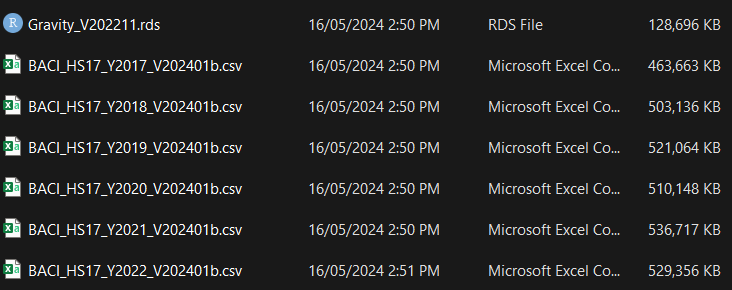
\includegraphics{pic1.png}

Notes about the data country\_codes, product\_codes and Readme are all
for reading BACI.

\hypertarget{packages}{%
\subsection{Packages}\label{packages}}

for this page I use these packages but you may not need all of them

\begin{Shaded}
\begin{Highlighting}[numbers=left,,]
\FunctionTok{library}\NormalTok{(tidyverse)}
\FunctionTok{library}\NormalTok{(penppml) }\DocumentationTok{\#\# no need}
\FunctionTok{library}\NormalTok{(writexl)}
\FunctionTok{library}\NormalTok{(modelsummary) }\DocumentationTok{\#\# no need}
\FunctionTok{library}\NormalTok{(gravity)}
\end{Highlighting}
\end{Shaded}

\hypertarget{simple-gravity-specification}{%
\section{Simple gravity
specification}\label{simple-gravity-specification}}

\hypertarget{theory}{%
\subsection{Theory}\label{theory}}

The earliest (e.g., naive) gravity model taking directly from Newtonian
gravity theory looks something like this:

\begin{equation}\protect\hypertarget{eq-1}{}{
X_{ij}=\tilde{G}\frac{Y_iE_j}{T_{ij}^\theta}
}\label{eq-1}\end{equation}

where \(X_{it}\) is the value of trade flow from country \(i\) to
country \(j\), \(\tilde{G}\) is the gravitational constant (aka our
usual constant), \(Y_i\) is the output in country \(i\) \(E_j\) is the
value of expenditure in country \(j\) and \(T_{ij}\) is the total
bilateral trade frictions / trade cost between country \(i\) and country
\(j\).

There are various other types of gravity equations, but let's start with
a relatively simple one. One of my favorite simple gravity specification
is a budget version of Silva and Tenreyro (2006) which is taken from
Anderson and Wincoop (2003) which looks like this:

\begin{equation}\protect\hypertarget{eq-2}{}{
X_{ij}=\alpha_0 Y_i^{\alpha_1}Y_j^{\alpha_2}D_{ij}^{\alpha_3}e^{\theta_id_i+\theta_jd_j}
}\label{eq-2}\end{equation}

where \(\alpha_0\) is your \(\tilde{G}\), while \(Y\) is the output and
expenditure which is proxied with GDP. \(D_{ij}\) is the distance
between the two countries, which can be generalized as a vector of trade
cost measures. Typically we use physical distance but also other types
of bilateral trade cost. Lastly, the \(d_i\) and \(d_j\) is
country-specific characteristics.

There are various variables used in Silva and Tenreyro (2006). log of
exporter's and importer's GDP and GDP per capita. Various ``distance''
variables is used as well e.g., physical distance and variables like
contiguity, common-language dummy, colonial-tie dummy and free trade
agreement dummy.

Note that our regression consists only of two indices: exporter \(i\)
and importer \(j\). We are going to use the gravity data I mentioned
earlier, slice the dataset to cover only one year chosen arbitrarily
(which is 2019), and run Equation~\ref{eq-2}.

\hypertarget{setting-data}{%
\subsection{Setting data}\label{setting-data}}

first we load all the necessary data:

\begin{Shaded}
\begin{Highlighting}[numbers=left,,]
\DocumentationTok{\#\# Readubg data}
\NormalTok{gravity }\OtherTok{\textless{}{-}} \FunctionTok{readRDS}\NormalTok{(}\StringTok{"Gravity\_V202211.rds"}\NormalTok{)}
\NormalTok{key}\OtherTok{\textless{}{-}}\FunctionTok{read\_csv}\NormalTok{(}\StringTok{"country\_codes\_V202401b.csv"}\NormalTok{)}
\end{Highlighting}
\end{Shaded}

The gravity is the data from CEPII while key is storing some country
codes. You can see the first 10 rows of the data and its variable names
you call their name. Just type \texttt{gravity} or \texttt{key} in the
console then hit enter. However, if you just want to look at the
variable names, you can use \texttt{colnames()}

\begin{Shaded}
\begin{Highlighting}[]
\FunctionTok{colnames}\NormalTok{(gravity)}
\end{Highlighting}
\end{Shaded}

\begin{verbatim}
 [1] "year"                   "country_id_o"           "country_id_d"          
 [4] "iso3_o"                 "iso3_d"                 "iso3num_o"             
 [7] "iso3num_d"              "country_exists_o"       "country_exists_d"      
[10] "gmt_offset_2020_o"      "gmt_offset_2020_d"      "distw_harmonic"        
[13] "distw_arithmetic"       "distw_harmonic_jh"      "distw_arithmetic_jh"   
[16] "dist"                   "main_city_source_o"     "main_city_source_d"    
[19] "distcap"                "contig"                 "diplo_disagreement"    
[22] "scaled_sci_2021"        "comlang_off"            "comlang_ethno"         
[25] "comcol"                 "col45"                  "legal_old_o"           
[28] "legal_old_d"            "legal_new_o"            "legal_new_d"           
[31] "comleg_pretrans"        "comleg_posttrans"       "transition_legalchange"
[34] "comrelig"               "heg_o"                  "heg_d"                 
[37] "col_dep_ever"           "col_dep"                "col_dep_end_year"      
[40] "col_dep_end_conflict"   "empire"                 "sibling_ever"          
[43] "sibling"                "sever_year"             "sib_conflict"          
[46] "pop_o"                  "pop_d"                  "gdp_o"                 
[49] "gdp_d"                  "gdpcap_o"               "gdpcap_d"              
[52] "pop_source_o"           "pop_source_d"           "gdp_source_o"          
[55] "gdp_source_d"           "gdp_ppp_o"              "gdp_ppp_d"             
[58] "gdpcap_ppp_o"           "gdpcap_ppp_d"           "pop_pwt_o"             
[61] "pop_pwt_d"              "gdp_ppp_pwt_o"          "gdp_ppp_pwt_d"         
[64] "gatt_o"                 "gatt_d"                 "wto_o"                 
[67] "wto_d"                  "eu_o"                   "eu_d"                  
[70] "fta_wto"                "fta_wto_raw"            "rta_coverage"          
[73] "rta_type"               "entry_cost_o"           "entry_cost_d"          
[76] "entry_proc_o"           "entry_proc_d"           "entry_time_o"          
[79] "entry_time_d"           "entry_tp_o"             "entry_tp_d"            
[82] "tradeflow_comtrade_o"   "tradeflow_comtrade_d"   "tradeflow_baci"        
[85] "manuf_tradeflow_baci"   "tradeflow_imf_o"        "tradeflow_imf_d"       
\end{verbatim}

As you can see, the column names are so plenty. Consult to the CEPII
website or Conte, Cotterlaz, and Mayer (2022) to learn more. We will
only use some of them, so we will filter these data to make it more
concise. Specifically, we will (1) remove some countries, (2) remove
non-2019, and (3) remove variables we are not using.

For variables, we will keep iso3\_o, iso3\_d, distw\_harmonic, contig,
comcol, comlang\_off,gdp\_o,gdp\_d, gdpcap\_o, gdpcap\_d,fta\_wto. Note
that o means origin / exporter and d means destination / importer.

\begin{Shaded}
\begin{Highlighting}[numbers=left,,]
\DocumentationTok{\#\# create a country list}
\NormalTok{ctr}\OtherTok{\textless{}{-}}\FunctionTok{c}\NormalTok{(}\StringTok{"Albania"}\NormalTok{, }\StringTok{"Denmark"}\NormalTok{, }\StringTok{"Kenya"}\NormalTok{, }\StringTok{"Romania"}\NormalTok{, }\StringTok{"Algeria"}\NormalTok{, }\StringTok{"Djibouti"}\NormalTok{, }\StringTok{"Kiribati"}\NormalTok{, }\StringTok{"Russian Federation"}\NormalTok{, }\StringTok{"Angola"}\NormalTok{, }\StringTok{"Dominican Rep."}\NormalTok{, }\StringTok{"Korea, Rep."}\NormalTok{, }\StringTok{"Rwanda"}\NormalTok{, }\StringTok{"Argentina"}\NormalTok{, }\StringTok{"Ecuador"}\NormalTok{, }\StringTok{"Laos"}\NormalTok{, }\StringTok{"P. Dem. Rep."}\NormalTok{, }\StringTok{"Saudi Arabia"}\NormalTok{, }\StringTok{"Australia"}\NormalTok{, }\StringTok{"Egypt"}\NormalTok{, }\StringTok{"Lebanon"}\NormalTok{, }\StringTok{"Senegal"}\NormalTok{, }\StringTok{"Austria"}\NormalTok{, }\StringTok{"El Salvador"}\NormalTok{, }\StringTok{"Madagascar"}\NormalTok{, }\StringTok{"Seychelles"}\NormalTok{, }\StringTok{"Bahamas"}\NormalTok{, }\StringTok{"Eq. Guinea"}\NormalTok{, }\StringTok{"Malawi"}\NormalTok{, }\StringTok{"Sierra Leone"}\NormalTok{, }\StringTok{"Bahrain"}\NormalTok{, }\StringTok{"Ethiopia"}\NormalTok{, }\StringTok{"Malaysia"}\NormalTok{, }\StringTok{"Singapore"}\NormalTok{, }\StringTok{"Bangladesh"}\NormalTok{, }\StringTok{"Fiji"}\NormalTok{, }\StringTok{"Maldives"}\NormalTok{, }\StringTok{"Solomon Islands"}\NormalTok{, }\StringTok{"Barbados"}\NormalTok{, }\StringTok{"Finland"}\NormalTok{, }\StringTok{"Mali"}\NormalTok{, }\StringTok{"South Africa"}\NormalTok{, }\StringTok{"Belgium{-}Lux."}\NormalTok{, }\StringTok{"France"}\NormalTok{, }\StringTok{"Malta"}\NormalTok{, }\StringTok{"Spain"}\NormalTok{, }\StringTok{"Belize"}\NormalTok{, }\StringTok{"Gabon"}\NormalTok{, }\StringTok{"Mauritania"}\NormalTok{, }\StringTok{"Sri Lanka"}\NormalTok{, }\StringTok{"Benin"}\NormalTok{, }\StringTok{"Gambia"}\NormalTok{, }\StringTok{"Mauritius"}\NormalTok{, }\StringTok{"St. Kitts and Nevis"}\NormalTok{, }\StringTok{"Bhutan"}\NormalTok{, }\StringTok{"Germany"}\NormalTok{, }\StringTok{"Mexico"}\NormalTok{, }\StringTok{"Sudan"}\NormalTok{, }\StringTok{"Bolivia"}\NormalTok{, }\StringTok{"Ghana"}\NormalTok{, }\StringTok{"Mongolia"}\NormalTok{, }\StringTok{"Suriname"}\NormalTok{, }\StringTok{"Brazil"}\NormalTok{, }\StringTok{"Greece"}\NormalTok{, }\StringTok{"Morocco"}\NormalTok{, }\StringTok{"Sweden"}\NormalTok{, }\StringTok{"Brunei"}\NormalTok{, }\StringTok{"Guatemala"}\NormalTok{, }\StringTok{"Mozambique"}\NormalTok{, }\StringTok{"Switzerland"}\NormalTok{, }\StringTok{"Bulgaria"}\NormalTok{, }\StringTok{"Guinea"}\NormalTok{, }\StringTok{"Nepal"}\NormalTok{, }\StringTok{"Syrian Arab Rep."}\NormalTok{, }\StringTok{"Burkina Faso"}\NormalTok{, }\StringTok{"Guinea{-}Bissau"}\NormalTok{, }\StringTok{"Netherlands"}\NormalTok{, }\StringTok{"Tanzania"}\NormalTok{, }\StringTok{"Burundi"}\NormalTok{, }\StringTok{"Guyana"}\NormalTok{, }\StringTok{"New Caledonia"}\NormalTok{, }\StringTok{"Thailand"}\NormalTok{, }\StringTok{"Cambodia"}\NormalTok{, }\StringTok{"Haiti"}\NormalTok{, }\StringTok{"New Zealand"}\NormalTok{, }\StringTok{"Togo"}\NormalTok{, }\StringTok{"Cameroon"}\NormalTok{, }\StringTok{"Honduras"}\NormalTok{, }\StringTok{"Nicaragua"}\NormalTok{, }\StringTok{"Trinidad and Tobago"}\NormalTok{, }\StringTok{"Canada"}\NormalTok{, }\StringTok{"Hong Kong"}\NormalTok{, }\StringTok{"Niger"}\NormalTok{, }\StringTok{"Tunisia"}\NormalTok{, }\StringTok{"Central African Rep."}\NormalTok{, }\StringTok{"Hungary"}\NormalTok{, }\StringTok{"Nigeria"}\NormalTok{, }\StringTok{"Turkey"}\NormalTok{, }\StringTok{"Chad"}\NormalTok{, }\StringTok{"Iceland"}\NormalTok{, }\StringTok{"Norway"}\NormalTok{, }\StringTok{"Uganda"}\NormalTok{, }\StringTok{"Chile"}\NormalTok{, }\StringTok{"India"}\NormalTok{, }\StringTok{"Oman"}\NormalTok{, }\StringTok{"United Arab Em."}\NormalTok{, }\StringTok{"China"}\NormalTok{, }\StringTok{"Indonesia"}\NormalTok{, }\StringTok{"Pakistan"}\NormalTok{, }\StringTok{"United Kingdom"}\NormalTok{, }\StringTok{"Colombia"}\NormalTok{, }\StringTok{"Iran"}\NormalTok{, }\StringTok{"Panama"}\NormalTok{, }\StringTok{"United States"}\NormalTok{, }\StringTok{"Comoros"}\NormalTok{, }\StringTok{"Ireland"}\NormalTok{, }\StringTok{"Papua New Guinea"}\NormalTok{, }\StringTok{"Uruguay"}\NormalTok{, }\StringTok{"Congo Dem. Rep."}\NormalTok{, }\StringTok{"Israel"}\NormalTok{, }\StringTok{"Paraguay"}\NormalTok{, }\StringTok{"Venezuela"}\NormalTok{, }\StringTok{"Congo Rep."}\NormalTok{, }\StringTok{"Italy"}\NormalTok{, }\StringTok{"Peru"}\NormalTok{, }\StringTok{"Vietnam"}\NormalTok{, }\StringTok{"Costa Rica"}\NormalTok{, }\StringTok{"Jamaica"}\NormalTok{, }\StringTok{"Philippines"}\NormalTok{, }\StringTok{"Yemen"}\NormalTok{, }\StringTok{"Cote D’lvoire"}\NormalTok{, }\StringTok{"Japan"}\NormalTok{, }\StringTok{"Poland"}\NormalTok{, }\StringTok{"Zambia"}\NormalTok{, }\StringTok{"Cyprus"}\NormalTok{, }\StringTok{"Jordan"}\NormalTok{, }\StringTok{"Portugal"}\NormalTok{, }\StringTok{"Zimbabwe"}\NormalTok{)}

\NormalTok{vrb}\OtherTok{\textless{}{-}}\FunctionTok{c}\NormalTok{(}\StringTok{"iso3num\_o"}\NormalTok{,}\StringTok{"iso3num\_d"}\NormalTok{,}\StringTok{"year"}\NormalTok{,}\StringTok{"iso3\_o"}\NormalTok{, }\StringTok{"iso3\_d"}\NormalTok{, }\StringTok{"distw\_harmonic"}\NormalTok{, }\StringTok{"contig"}\NormalTok{, }\StringTok{"comcol"}\NormalTok{, }\StringTok{"comlang\_off"}\NormalTok{,}\StringTok{"gdp\_o"}\NormalTok{,}\StringTok{"gdp\_d"}\NormalTok{, }\StringTok{"gdpcap\_o"}\NormalTok{, }\StringTok{"gdpcap\_d"}\NormalTok{,}\StringTok{"fta\_wto"}\NormalTok{,}\StringTok{"tradeflow\_baci"}\NormalTok{)}

\DocumentationTok{\#\# keep 2019}
\NormalTok{gravity2}\OtherTok{\textless{}{-}}\NormalTok{gravity}\SpecialCharTok{|\textgreater{}}\FunctionTok{filter}\NormalTok{(year}\SpecialCharTok{==}\DecValTok{2019}\NormalTok{)}

\DocumentationTok{\#\# Keep countries in the list}
\NormalTok{key2}\OtherTok{\textless{}{-}}\NormalTok{key }\SpecialCharTok{|\textgreater{}} \FunctionTok{filter}\NormalTok{(country\_name}\SpecialCharTok{\%in\%}\NormalTok{ctr)}
\NormalTok{gravity2}\OtherTok{\textless{}{-}}\NormalTok{gravity2 }\SpecialCharTok{|\textgreater{}} \FunctionTok{filter}\NormalTok{(country\_id\_o }\SpecialCharTok{\%in\%}\NormalTok{ key2}\SpecialCharTok{$}\NormalTok{country\_iso3 }\SpecialCharTok{\&}\NormalTok{ country\_id\_d }\SpecialCharTok{\%in\%}\NormalTok{ key2}\SpecialCharTok{$}\NormalTok{country\_iso3)}
\NormalTok{gravity2}\OtherTok{\textless{}{-}}\NormalTok{gravity2 }\SpecialCharTok{|\textgreater{}} \FunctionTok{select}\NormalTok{(vrb)}

\DocumentationTok{\#\# Make a log versin}
\NormalTok{gravity2}\OtherTok{\textless{}{-}}\NormalTok{gravity2 }\SpecialCharTok{|\textgreater{}}
  \FunctionTok{mutate}\NormalTok{(}\AttributeTok{ldist=}\FunctionTok{log}\NormalTok{(distw\_harmonic),}
         \AttributeTok{lgdpo=}\FunctionTok{log}\NormalTok{(gdp\_o),}
         \AttributeTok{lgdpd=}\FunctionTok{log}\NormalTok{(gdp\_d),}
         \AttributeTok{lgdpco=}\FunctionTok{log}\NormalTok{(gdpcap\_o),}
         \AttributeTok{lgdpcd=}\FunctionTok{log}\NormalTok{(gdpcap\_d),}
         \AttributeTok{logtrade=}\FunctionTok{log}\NormalTok{(}\DecValTok{1}\SpecialCharTok{+}\NormalTok{tradeflow\_baci))}
\end{Highlighting}
\end{Shaded}

You can see in your environment tab the difference between gravity and
gravity2 as well as between key and key2 on the number of observations
and variables. Note that we also log non-dummy variables for gravity2 to
redo Silva and Tenreyro (2006).

We will focus on the gravity2 as it will be the dataset we will run. You
can quickly show summary statistics by typing \texttt{summary(gravity2)}
on the console tab.

\begin{Shaded}
\begin{Highlighting}[]
\FunctionTok{summary}\NormalTok{(gravity2)}
\end{Highlighting}
\end{Shaded}

\begin{verbatim}
   iso3num_o       iso3num_d          year         iso3_o         
 Min.   :  8.0   Min.   :  8.0   Min.   :2019   Length:12321      
 1st Qu.:204.0   1st Qu.:204.0   1st Qu.:2019   Class :character  
 Median :400.0   Median :400.0   Median :2019   Mode  :character  
 Mean   :415.5   Mean   :415.5   Mean   :2019                     
 3rd Qu.:616.0   3rd Qu.:616.0   3rd Qu.:2019                     
 Max.   :894.0   Max.   :894.0   Max.   :2019                     
                                                                  
    iso3_d          distw_harmonic      contig            comcol       
 Length:12321       Min.   :    4   Min.   :0.00000   Min.   :0.00000  
 Class :character   1st Qu.: 4459   1st Qu.:0.00000   1st Qu.:0.00000  
 Mode  :character   Median : 7587   Median :0.00000   Median :0.00000  
                    Mean   : 7932   Mean   :0.01753   Mean   :0.09739  
                    3rd Qu.:11024   3rd Qu.:0.00000   3rd Qu.:0.00000  
                    Max.   :19676   Max.   :1.00000   Max.   :1.00000  
                                                                       
  comlang_off         gdp_o               gdp_d              gdpcap_o     
 Min.   :0.0000   Min.   :1.779e+05   Min.   :1.779e+05   Min.   : 0.224  
 1st Qu.:0.0000   1st Qu.:1.419e+07   1st Qu.:1.419e+07   1st Qu.: 1.909  
 Median :0.0000   Median :4.805e+07   Median :4.805e+07   Median : 6.321  
 Mean   :0.1789   Mean   :4.785e+08   Mean   :4.785e+08   Mean   :15.262  
 3rd Qu.:0.0000   3rd Qu.:3.512e+08   3rd Qu.:3.512e+08   3rd Qu.:18.480  
 Max.   :1.0000   Max.   :1.428e+10   Max.   :1.428e+10   Max.   :85.335  
                  NA's   :111         NA's   :111         NA's   :111     
    gdpcap_d         fta_wto       tradeflow_baci          ldist      
 Min.   : 0.224   Min.   :0.0000   Min.   :        0   Min.   :1.386  
 1st Qu.: 1.909   1st Qu.:0.0000   1st Qu.:      273   1st Qu.:8.403  
 Median : 6.321   Median :0.0000   Median :     6343   Median :8.934  
 Mean   :15.262   Mean   :0.2023   Mean   :   611172   Mean   :8.721  
 3rd Qu.:18.480   3rd Qu.:0.0000   3rd Qu.:    87003   3rd Qu.:9.308  
 Max.   :85.335   Max.   :1.0000   Max.   :149568313   Max.   :9.887  
 NA's   :111                       NA's   :2185                       
     lgdpo           lgdpd           lgdpco            lgdpcd       
 Min.   :12.09   Min.   :12.09   Min.   :-1.4961   Min.   :-1.4961  
 1st Qu.:16.47   1st Qu.:16.47   1st Qu.: 0.6466   1st Qu.: 0.6466  
 Median :17.69   Median :17.69   Median : 1.8438   Median : 1.8438  
 Mean   :17.93   Mean   :17.93   Mean   : 1.8087   Mean   : 1.8087  
 3rd Qu.:19.68   3rd Qu.:19.68   3rd Qu.: 2.9167   3rd Qu.: 2.9167  
 Max.   :23.38   Max.   :23.38   Max.   : 4.4466   Max.   : 4.4466  
 NA's   :111     NA's   :111     NA's   :111       NA's   :111      
    logtrade     
 Min.   : 0.001  
 1st Qu.: 5.613  
 Median : 8.755  
 Mean   : 8.438  
 3rd Qu.:11.374  
 Max.   :18.823  
 NA's   :2185    
\end{verbatim}

\hypertarget{regression}{%
\subsection{Regression}\label{regression}}

Let's do 2 types of regression. First we do a regression using a normal
ols, and secondly we do ppml.

\begin{Shaded}
\begin{Highlighting}[]
\NormalTok{reg1}\OtherTok{\textless{}{-}}\FunctionTok{lm}\NormalTok{(logtrade}\SpecialCharTok{\textasciitilde{}}\NormalTok{lgdpo}\SpecialCharTok{+}\NormalTok{lgdpd}\SpecialCharTok{+}\NormalTok{lgdpco}\SpecialCharTok{+}\NormalTok{lgdpcd}\SpecialCharTok{+}\NormalTok{ldist}\SpecialCharTok{+}\NormalTok{contig}\SpecialCharTok{+}\NormalTok{comcol}\SpecialCharTok{+}\NormalTok{comlang\_off}\SpecialCharTok{+}\NormalTok{fta\_wto)}
\NormalTok{reg2}\OtherTok{\textless{}{-}}\FunctionTok{lm}\NormalTok{(logtrade}\SpecialCharTok{\textasciitilde{}}\NormalTok{lgdpo}\SpecialCharTok{+}\NormalTok{lgdpd}\SpecialCharTok{+}\NormalTok{lgdpco}\SpecialCharTok{+}\NormalTok{lgdpcd}\SpecialCharTok{+}\NormalTok{ldist}\SpecialCharTok{+}\NormalTok{contig}\SpecialCharTok{+}\NormalTok{comcol}\SpecialCharTok{+}\NormalTok{comlang\_off}\SpecialCharTok{+}\NormalTok{fta\_wto}\SpecialCharTok{+}\NormalTok{iso3\_o}\SpecialCharTok{+}\NormalTok{iso3\_d)}
\NormalTok{reg3}\OtherTok{\textless{}{-}}\FunctionTok{ppml}\NormalTok{(}\AttributeTok{data=}\NormalTok{gravity2,}\AttributeTok{dependent\_variable=}\StringTok{"tradeflow\_baci"}\NormalTok{,}\AttributeTok{distance=}\StringTok{"distw\_harmonic"}\NormalTok{,}\AttributeTok{additional\_regressors=}\FunctionTok{c}\NormalTok{(}\StringTok{"lgdpo"}\NormalTok{,}\StringTok{"lgdpd"}\NormalTok{,}\StringTok{"lgdpco"}\NormalTok{,}\StringTok{"lgdpcd"}\NormalTok{,}\StringTok{"contig"}\NormalTok{,}\StringTok{"comcol"}\NormalTok{,}\StringTok{"comlang\_off"}\NormalTok{,}\StringTok{"fta\_wto"}\NormalTok{))}
\NormalTok{reg4}\OtherTok{\textless{}{-}}\FunctionTok{ppml}\NormalTok{(}\AttributeTok{data=}\NormalTok{gravity2,}\AttributeTok{dependent\_variable=}\StringTok{"tradeflow\_baci"}\NormalTok{,}\AttributeTok{distance=}\StringTok{"distw\_harmonic"}\NormalTok{,}\AttributeTok{additional\_regressors=}\FunctionTok{c}\NormalTok{(}\StringTok{"lgdpo"}\NormalTok{,}\StringTok{"lgdpd"}\NormalTok{,}\StringTok{"lgdpco"}\NormalTok{,}\StringTok{"lgdpcd"}\NormalTok{,}\StringTok{"contig"}\NormalTok{,}\StringTok{"comcol"}\NormalTok{,}\StringTok{"comlang\_off"}\NormalTok{,}\StringTok{"fta\_wto"}\NormalTok{,}\StringTok{"iso3\_o"}\NormalTok{,}\StringTok{"iso3\_d"}\NormalTok{))}
\end{Highlighting}
\end{Shaded}

You can call each reg's table with \texttt{summary(reg1)}.

\begin{table}
\caption{Simple regression results}\tabularnewline

\centering
\begin{talltblr}[         %% tabularray outer open
entry=none,label=none,
note{}={+ p < 0.1, * p < 0.05, ** p < 0.01, *** p < 0.001},
]                     %% tabularray outer close
{                     %% tabularray inner open
colspec={Q[]Q[]Q[]Q[]Q[]},
column{1}={halign=l,},
column{2}={halign=c,},
column{3}={halign=c,},
column{4}={halign=c,},
column{5}={halign=c,},
hline{24}={1,2,3,4,5}{solid, 0.05em, black},
}                     %% tabularray inner close
\toprule
& OLS no ctr & OLS with ctr & PPML no ctr & PPML with ctr \\ \midrule %% TinyTableHeader
(Intercept)   & \num{-21.866}*** & \num{-81.921}**  & \num{-15.380}*** & \num{-118.218}*  \\
& (\num{0.414})    & (\num{30.733})   & (\num{0.255})    & (\num{49.820})   \\
lgdpo         & \num{1.239}***   & \num{1.739}      & \num{0.895}***   & \num{6.704}**    \\
& (\num{0.013})    & (\num{1.367})    & (\num{0.008})    & (\num{2.374})    \\
lgdpd         & \num{0.947}***   & \num{4.220}**    & \num{0.814}***   & \num{1.349}      \\
& (\num{0.013})    & (\num{1.285})    & (\num{0.008})    & (\num{1.884})    \\
lgdpco        & \num{0.251}***   & \num{-2.090}     & \num{-0.041}***  & \num{-10.947}*   \\
& (\num{0.018})    & (\num{3.196})    & (\num{0.012})    & (\num{5.283})    \\
lgdpcd        & \num{0.066}***   & \num{-6.527}*    & \num{-0.037}**   & \num{-1.280}     \\
& (\num{0.018})    & (\num{2.996})    & (\num{0.011})    & (\num{4.393})    \\
contig        & \num{0.899}***   & \num{0.594}***   & \num{0.185}***   & \num{0.334}***   \\
& (\num{0.165})    & (\num{0.147})    & (\num{0.037})    & (\num{0.031})    \\
comcol        & \num{0.489}***   & \num{0.317}***   & \num{0.110}      & \num{0.519}***   \\
& (\num{0.082})    & (\num{0.082})    & (\num{0.090})    & (\num{0.074})    \\
comlang\_off & \num{0.781}***   & \num{0.778}***   & \num{0.238}***   & \num{0.162}***   \\
& (\num{0.061})    & (\num{0.061})    & (\num{0.035})    & (\num{0.031})    \\
fta\_wto     & \num{0.702}***   & \num{0.559}***   & \num{0.383}***   & \num{0.380}***   \\
& (\num{0.057})    & (\num{0.057})    & (\num{0.028})    & (\num{0.025})    \\
ldist         & \num{-1.215}***  & \num{-1.466}***  &                   &                   \\
& (\num{0.032})    & (\num{0.032})    &                   &                   \\
dist\_log    &                   &                   & \num{-0.606}***  & \num{-0.711}***  \\
&                   &                   & (\num{0.013})    & (\num{0.012})    \\
Num.Obs.      & \num{9990}       & \num{9990}       & \num{9990}       & \num{9990}       \\
R2            & \num{0.720}      & \num{0.798}      &                   &                   \\
R2 Adj.       & \num{0.720}      & \num{0.793}      &                   &                   \\
AIC           & \num{43230.2}    & \num{40397.2}    &                   &                   \\
BIC           & \num{43309.5}    & \num{42019.3}    &                   &                   \\
Log.Lik.      & \num{-21604.098} & \num{-19973.582} &                   &                   \\
RMSE          & \num{2.10}       & \num{1.79}       & \num{2097486.21} & \num{1585545.74} \\
\bottomrule
\end{talltblr}
\end{table}

You can compare results with Silva and Tenreyro (2006). Note that they
don't use fixed effects.

\begin{figure}

{\centering 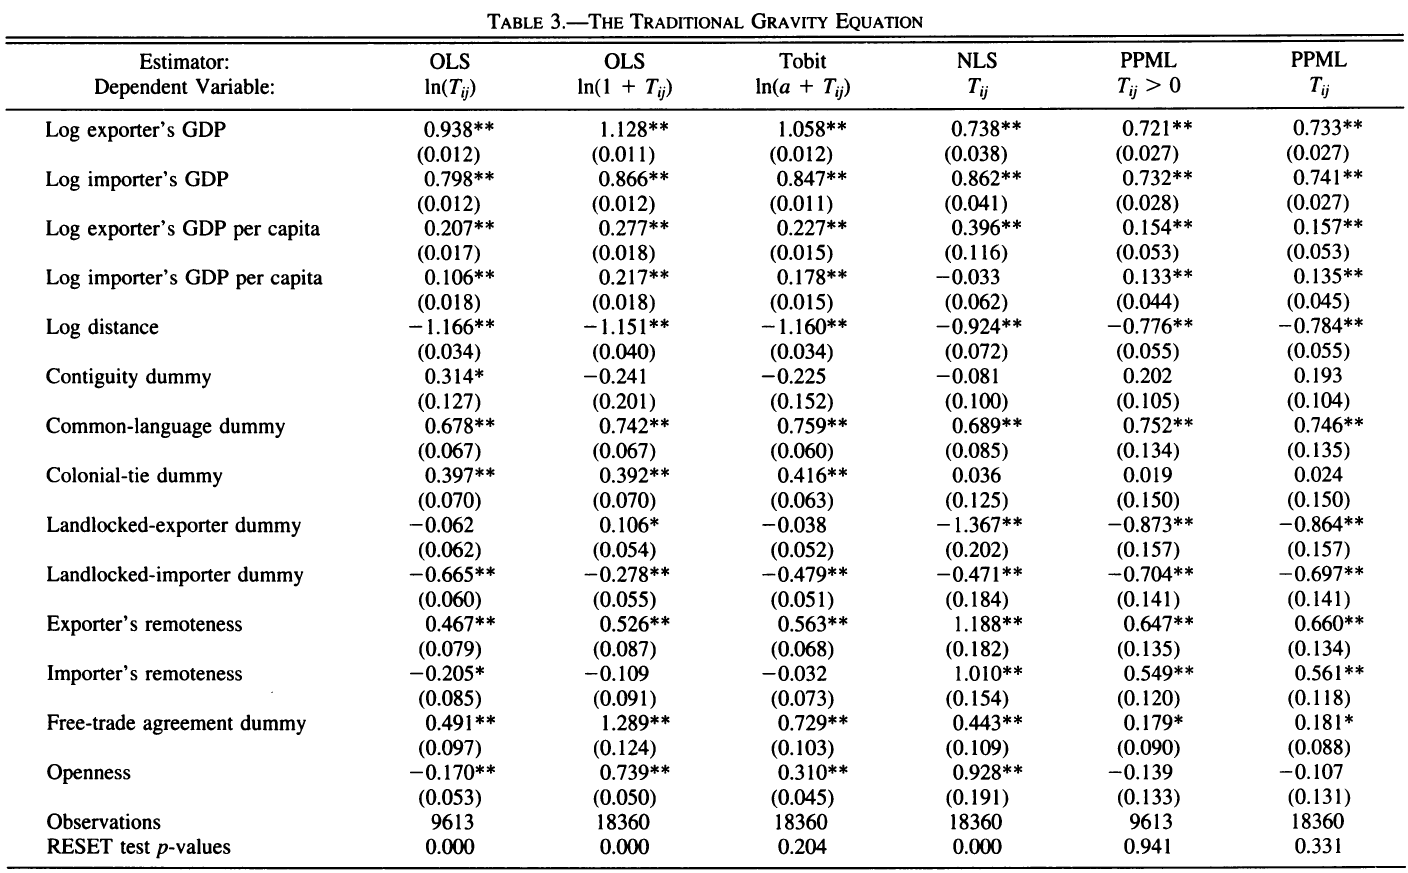
\includegraphics{pic2.png}

}

\caption{source: Silva and Tenreyro (2006)}

\end{figure}

By the way, you can save the regression table using
\texttt{modelsummary()}. don't forget to run
\texttt{library(modelsummary)} first. You can use xls extension, but
also doc. I personally like .html more.

\begin{Shaded}
\begin{Highlighting}[]
\NormalTok{regtab}\OtherTok{\textless{}{-}} \FunctionTok{list}\NormalTok{(}
  \StringTok{"OLS no ctr"} \OtherTok{=}\NormalTok{ reg1,}
  \StringTok{"OLS with ctr"}  \OtherTok{=}\NormalTok{ reg2,}
  \StringTok{"PPML no ctr"}\OtherTok{=}\NormalTok{reg3,}
  \StringTok{"PPML with ctr"}\OtherTok{=}\NormalTok{reg4}
\NormalTok{)}
\FunctionTok{modelsummary}\NormalTok{(regtab,}\AttributeTok{output=}\StringTok{"regtab.xls"}\NormalTok{)}
\end{Highlighting}
\end{Shaded}

\hypertarget{product-level-gravity}{%
\section{Product level gravity}\label{product-level-gravity}}

\hypertarget{theory-1}{%
\subsection{Theory}\label{theory-1}}

We then proceed to a higher-dimension trade data which you may be
interested in. In the field, UI students often interested largely in
Indonesian affairs. That is, we are not interested so much in the
bilateral flow of all countries, but only on Indonesia. However, we
often use more granular dimension than just exporter/importer. Often
times we use indices like time, commodities or industries, or even firms
(shamelessly inserting my paper here Gupta (2023)).

Now, if you are planning to do these kinds of studies, then you are
going to need to tackle higher degree dataset and merging the gravity
variables. Most often you can get these variables from
\href{https://databank.worldbank.org/source/world-development-indicators}{World
Development Indicators} but CEPII is ok for now (note the main problem
of CEPII is its timeliness).

The theory isn't so different compared to our previous gravity model.
What we want is an additional indices. We are going to estimate
something similar as Equation~\ref{eq-2} but with more indices. We need
to care about multilateral resistance (MR) and we can use dummies since
we now have more variations from indices like time and HS code.

According to Yotov (2022), we need at least 3 dummies to run a
multi-country, multi-time and multi-goods/sectors\footnote{unless you
  have domestic trade data which we typically don't. If you do, then
  there's borders dummy. More on Yotov (2022).}. We need to have
exporter-time dummy, importer-time dummy and country-pair dummy. We need
to construct this first. Note that these dummies will likely absorb some
of your variables like distance (consistant between pair across time,
typically).

So we will do the HS,time varying version of Equation~\ref{eq-2}:

\begin{equation}\protect\hypertarget{eq-3}{}{
X_{ijpt}=\alpha_0 Y_{it}^{\alpha_1}Y_{jt}^{\alpha_2}D_{ijpt}^{\alpha_3}e^{\theta_1o_{it}+\theta_2d_{jt}+\theta_3p_{ij}}
}\label{eq-3}\end{equation}

\hypertarget{setting-data-1}{%
\subsection{Setting data}\label{setting-data-1}}

This time we need BACI data. Brace yourself because this dataset is
HUGE. We read 5 different years.

\begin{Shaded}
\begin{Highlighting}[numbers=left,,]
\NormalTok{t2017}\OtherTok{\textless{}{-}}\FunctionTok{read\_csv}\NormalTok{(}\StringTok{"BACI\_HS17\_Y2017\_V202401b.csv"}\NormalTok{)}
\NormalTok{t2018}\OtherTok{\textless{}{-}}\FunctionTok{read\_csv}\NormalTok{(}\StringTok{"BACI\_HS17\_Y2018\_V202401b.csv"}\NormalTok{)}
\NormalTok{t2019}\OtherTok{\textless{}{-}}\FunctionTok{read\_csv}\NormalTok{(}\StringTok{"BACI\_HS17\_Y2019\_V202401b.csv"}\NormalTok{)}
\NormalTok{t2020}\OtherTok{\textless{}{-}}\FunctionTok{read\_csv}\NormalTok{(}\StringTok{"BACI\_HS17\_Y2020\_V202401b.csv"}\NormalTok{)}
\NormalTok{t2021}\OtherTok{\textless{}{-}}\FunctionTok{read\_csv}\NormalTok{(}\StringTok{"BACI\_HS17\_Y2021\_V202401b.csv"}\NormalTok{)}


\DocumentationTok{\#\# Combining all }
\NormalTok{trade}\OtherTok{\textless{}{-}}\FunctionTok{rbind}\NormalTok{(t2017,t2018,t2019,t2020,t2021)}

\FunctionTok{remove}\NormalTok{(t2017,t2018,t2019,t2020,t2021)}
\end{Highlighting}
\end{Shaded}

I used \texttt{read\_csv} from the tydiverse package for reading .csv.
rbind is to stack all BACI data (it was separated per year), then I
remove the individual BACI to save environment space.

At this point, you can try checking out the two datasets. You can try
looking at both data by calling their names. Alternatively, just look at
the column names with \texttt{colnames()}. Let's try the BACI frist.

\begin{Shaded}
\begin{Highlighting}[]
\FunctionTok{colnames}\NormalTok{(trade)}
\end{Highlighting}
\end{Shaded}

\begin{verbatim}
[1] "t" "i" "j" "k" "v" "q"
\end{verbatim}

There are only 6 columns / variables. Here's some information on what
thos means

\begin{longtable}[]{@{}ll@{}}
\toprule\noalign{}
var & meaning \\
\midrule\noalign{}
\endhead
\bottomrule\noalign{}
\endlastfoot
t & year \\
i & exporter \\
j & importer \\
k & product \\
v & value \\
q & quantity \\
\end{longtable}

Products in Harmonized System 6-digit nomenclature. Values in thousand
USD and quantities in metric tons. Exporter and importer is codified
using CEPII codes. the codes and it means can be found in the ``key''
dataset. To have country identities into the BACI dataset, we need to
join the two.

To join the two datasets, we need a key variable. A key variable is the
variable connecting the two variables. Both needs the same name. So
first we need to assign the same name for exporter and importer codes
between BACI and gravity.

We know that \(i\) in BACI is iso3num\_o in gravity, while \(j\) in BACI
is iso3num\_d in gravity. So we rename the one in BACI so both have the
same name:

\begin{Shaded}
\begin{Highlighting}[numbers=left,,]
\DocumentationTok{\#\# Rename variable}
\NormalTok{trade2}\OtherTok{\textless{}{-}}\NormalTok{trade}\SpecialCharTok{|\textgreater{}}\FunctionTok{rename}\NormalTok{(}\AttributeTok{iso3num\_o=}\NormalTok{i,}\AttributeTok{iso3num\_d=}\NormalTok{j,}\AttributeTok{year=}\NormalTok{t)}

\DocumentationTok{\#\# Change ctr to reduce computation problem}
\NormalTok{ctr}\OtherTok{\textless{}{-}}\FunctionTok{c}\NormalTok{(}\StringTok{"IDN"}\NormalTok{,}\StringTok{"SGP"}\NormalTok{,}\StringTok{"VNM"}\NormalTok{,}\StringTok{"MYS"}\NormalTok{,}\StringTok{"THA"}\NormalTok{,}\StringTok{"PHL"}\NormalTok{,}\StringTok{"USA"}\NormalTok{,}\StringTok{"CHN"}\NormalTok{)}

\DocumentationTok{\#\# Kita ulangi gravity2 karena sekarang perlu tahun 2017{-}2021}
\NormalTok{gravity2}\OtherTok{\textless{}{-}}\NormalTok{gravity}\SpecialCharTok{|\textgreater{}}\FunctionTok{filter}\NormalTok{(year}\SpecialCharTok{\textgreater{}}\DecValTok{2016} \SpecialCharTok{\&}\NormalTok{ year}\SpecialCharTok{\textless{}}\DecValTok{2022}\NormalTok{)}
\NormalTok{gravity2}\OtherTok{\textless{}{-}}\NormalTok{gravity2 }\SpecialCharTok{|\textgreater{}} \FunctionTok{filter}\NormalTok{(iso3\_o }\SpecialCharTok{\%in\%}\NormalTok{ctr }\SpecialCharTok{\&}\NormalTok{ iso3\_d }\SpecialCharTok{\%in\%}\NormalTok{ ctr) }\DocumentationTok{\#\# notice the change}
\NormalTok{gravity2}\OtherTok{\textless{}{-}}\NormalTok{gravity2 }\SpecialCharTok{|\textgreater{}} \FunctionTok{select}\NormalTok{(vrb)}

\DocumentationTok{\#\# gabung dengan trade2}

\NormalTok{gabung}\OtherTok{\textless{}{-}}\FunctionTok{left\_join}\NormalTok{(gravity2,trade2,}\AttributeTok{by=}\FunctionTok{c}\NormalTok{(}\StringTok{"year"}\NormalTok{,}\StringTok{"iso3num\_o"}\NormalTok{,}\StringTok{"iso3num\_d"}\NormalTok{))}
\end{Highlighting}
\end{Shaded}

Check the results with gabung or \texttt{View(gabung)}. The most
important thing here is that you have to make sure you understand the
changes in variations! Now that we have time and HS (\(k\)), a pair of
countries can have multiple observations in different year and different
goods. tradeflow\_baci will be repeated because this is the total trade,
while now we focus on \(v\) and \(q\) as the \(X_{ijpt}\).

Before we go, however, we need to generate our dummies! Remember, we
need to make three dummies, \(o_{it}\),\(d_{jt}\) and \(p_{ij}\) (see
Equation~\ref{eq-3}). To do that, we do this:

\begin{Shaded}
\begin{Highlighting}[numbers=left,,]
\NormalTok{gabung }\OtherTok{\textless{}{-}}\NormalTok{ gabung }\SpecialCharTok{|\textgreater{}}
  \FunctionTok{mutate}\NormalTok{(}\AttributeTok{ooo=}\FunctionTok{interaction}\NormalTok{(iso3num\_o,year),}
         \AttributeTok{ddd=}\FunctionTok{interaction}\NormalTok{(iso3num\_d,year),}
         \AttributeTok{ppp=}\FunctionTok{interaction}\NormalTok{(iso3num\_o,iso3num\_d))}
\end{Highlighting}
\end{Shaded}

You can check again whether it's made. if you do \texttt{tibble(gabung)}
you will see that we have created our factor variables. Oh yes, do not
forget to log non-factors.

\begin{Shaded}
\begin{Highlighting}[numbers=left,,]
\NormalTok{gabung}\OtherTok{\textless{}{-}}\NormalTok{gabung }\SpecialCharTok{|\textgreater{}}
  \FunctionTok{mutate}\NormalTok{(}\AttributeTok{ldist=}\FunctionTok{log}\NormalTok{(distw\_harmonic),}
         \AttributeTok{lgdpo=}\FunctionTok{log}\NormalTok{(gdp\_o),}
         \AttributeTok{lgdpd=}\FunctionTok{log}\NormalTok{(gdp\_d),}
         \AttributeTok{lgdpco=}\FunctionTok{log}\NormalTok{(gdpcap\_o),}
         \AttributeTok{lgdpcd=}\FunctionTok{log}\NormalTok{(gdpcap\_d),}
         \AttributeTok{logtrade=}\FunctionTok{log}\NormalTok{(}\DecValTok{1}\SpecialCharTok{+}\NormalTok{v)) }\DocumentationTok{\#\# note the difference with before}
\end{Highlighting}
\end{Shaded}

\hypertarget{regression-1}{%
\subsection{Regression}\label{regression-1}}

\begin{Shaded}
\begin{Highlighting}[]
\NormalTok{ger1}\OtherTok{\textless{}{-}}\FunctionTok{lm}\NormalTok{(logtrade}\SpecialCharTok{\textasciitilde{}}\NormalTok{lgdpo}\SpecialCharTok{+}\NormalTok{lgdpd}\SpecialCharTok{+}\NormalTok{lgdpco}\SpecialCharTok{+}\NormalTok{lgdpcd}\SpecialCharTok{+}\NormalTok{ldist}\SpecialCharTok{+}\NormalTok{contig}\SpecialCharTok{+}\NormalTok{comcol}\SpecialCharTok{+}\NormalTok{comlang\_off}\SpecialCharTok{+}\NormalTok{fta\_wto)}
\NormalTok{ger2}\OtherTok{\textless{}{-}}\FunctionTok{lm}\NormalTok{(logtrade}\SpecialCharTok{\textasciitilde{}}\NormalTok{lgdpo}\SpecialCharTok{+}\NormalTok{lgdpd}\SpecialCharTok{+}\NormalTok{lgdpco}\SpecialCharTok{+}\NormalTok{lgdpcd}\SpecialCharTok{+}\NormalTok{ldist}\SpecialCharTok{+}\NormalTok{contig}\SpecialCharTok{+}\NormalTok{comcol}\SpecialCharTok{+}\NormalTok{comlang\_off}\SpecialCharTok{+}\NormalTok{fta\_wto}\SpecialCharTok{+}\NormalTok{iso3\_o}\SpecialCharTok{+}\NormalTok{iso3\_d)}
\NormalTok{ger3}\OtherTok{\textless{}{-}}\FunctionTok{ppml}\NormalTok{(}\AttributeTok{data=}\NormalTok{gravity2,}\AttributeTok{dependent\_variable=}\StringTok{"tradeflow\_baci"}\NormalTok{,}\AttributeTok{distance=}\StringTok{"distw\_harmonic"}\NormalTok{,}\AttributeTok{additional\_regressors=}\FunctionTok{c}\NormalTok{(}\StringTok{"lgdpo"}\NormalTok{,}\StringTok{"lgdpd"}\NormalTok{,}\StringTok{"lgdpco"}\NormalTok{,}\StringTok{"lgdpcd"}\NormalTok{,}\StringTok{"contig"}\NormalTok{,}\StringTok{"comcol"}\NormalTok{,}\StringTok{"comlang\_off"}\NormalTok{,}\StringTok{"fta\_wto"}\NormalTok{))}
\NormalTok{ger4}\OtherTok{\textless{}{-}}\FunctionTok{ppml}\NormalTok{(}\AttributeTok{data=}\NormalTok{gravity2,}\AttributeTok{dependent\_variable=}\StringTok{"tradeflow\_baci"}\NormalTok{,}\AttributeTok{distance=}\StringTok{"distw\_harmonic"}\NormalTok{,}\AttributeTok{additional\_regressors=}\FunctionTok{c}\NormalTok{(}\StringTok{"lgdpo"}\NormalTok{,}\StringTok{"lgdpd"}\NormalTok{,}\StringTok{"lgdpco"}\NormalTok{,}\StringTok{"lgdpcd"}\NormalTok{,}\StringTok{"contig"}\NormalTok{,}\StringTok{"comcol"}\NormalTok{,}\StringTok{"comlang\_off"}\NormalTok{,}\StringTok{"fta\_wto"}\NormalTok{,}\StringTok{"iso3\_o"}\NormalTok{,}\StringTok{"iso3\_d"}\NormalTok{))}
\end{Highlighting}
\end{Shaded}

\begin{table}
\caption{Simple regression results}\tabularnewline

\centering
\begin{talltblr}[         %% tabularray outer open
entry=none,label=none,
note{}={+ p < 0.1, * p < 0.05, ** p < 0.01, *** p < 0.001},
]                     %% tabularray outer close
{                     %% tabularray inner open
colspec={Q[]Q[]Q[]Q[]Q[]},
column{1}={halign=l,},
column{2}={halign=c,},
column{3}={halign=c,},
column{4}={halign=c,},
column{5}={halign=c,},
hline{22}={1,2,3,4,5}{solid, 0.05em, black},
}                     %% tabularray inner close
\toprule
& OLS no dum & OLS with dum & PPML no dum & PPML with dum \\ \midrule %% TinyTableHeader
(Intercept)   & \num{-12.184}***   & \num{-13.625}***   & \num{-9.350}*** & \num{1.137236e+10}   \\
& (\num{0.097})      & (\num{1.701})      & (\num{0.480})   & (\num{1.101188e+11}) \\
lgdpo         & \num{0.752}***     & \num{2.247}***     & \num{0.480}***  & \num{3.683411e+08}   \\
& (\num{0.003})      & (\num{0.359})      & (\num{0.017})   & (\num{9.301997e+08}) \\
lgdpd         & \num{0.165}***     & \num{-1.062}***    & \num{0.490}***  & \num{5.209835e+08}   \\
& (\num{0.003})      & (\num{0.153})      & (\num{0.017})   & (\num{3.745272e+09}) \\
lgdpco        & \num{-0.022}***    & \num{-0.754}***    & \num{-0.024}    & \num{-5.386022e+09}  \\
& (\num{0.005})      & (\num{0.176})      & (\num{0.027})   & (\num{1.351051e+10}) \\
lgdpcd        & \num{-0.228}***    & \num{-0.173}+      & \num{-0.006}    & \num{-9.331184e+09}  \\
& (\num{0.005})      & (\num{0.094})      & (\num{0.025})   & (\num{9.762501e+09}) \\
contig        & \num{0.517}***     & \num{0.151}*       & \num{0.588}***  & \num{1.841283e+09}   \\
& (\num{0.010})      & (\num{0.065})      & (\num{0.043})   & (\num{1.312649e+10}) \\
comcol        & \num{0.587}***     & \num{-0.565}       & \num{0.396}**   & \num{1.994991e+08}   \\
& (\num{0.029})      & (\num{0.999})      & (\num{0.139})   & (\num{2.047906e+10}) \\
comlang\_off & \num{0.415}***     & \num{0.310}        & \num{0.466}***  & \num{-2.140102e+09}  \\
& (\num{0.014})      & (\num{0.226})      & (\num{0.064})   & (\num{1.651348e+10}) \\
ldist         & \num{-0.232}***    & \num{-0.604}       &                  &                       \\
& (\num{0.010})      & (\num{0.478})      &                  &                       \\
dist\_log    &                     &                     & \num{-0.310}*** & \num{2.561000e+00}   \\
&                     &                     & (\num{0.056})   & (\num{2.410000e+00}) \\
Num.Obs.      & \num{613361}       & \num{613361}       & \num{613361}    & \num{613361}         \\
R2            & \num{0.123}        & \num{0.146}        &                  &                       \\
R2 Adj.       & \num{0.123}        & \num{0.146}        &                  &                       \\
AIC           & \num{2999982.1}    & \num{2984226.8}    &                  &                       \\
BIC           & \num{3000095.3}    & \num{2985314.2}    &                  &                       \\
Log.Lik.      & \num{-1499981.039} & \num{-1492017.404} &                  &                       \\
RMSE          & \num{2.79}         & \num{2.76}         & \num{90746.47}  & \num{90727.88}       \\
\bottomrule
\end{talltblr}
\end{table}

As you can see, the difference is apparent when we use HS-6-digit
instead of total trade. This is of course the case since now we have
wild, uncontrolled variability in the goods characteristics. Indeed, the
gravity equation is much better suited predicting total trade where
country and year characteristics dominates and industry/goods
heterogeneity is absorbed by the total trade. Remember, I use only small
number of countries with tons of HS 6 digit\footnote{I added CHN and USA
  in this version. Previously it was only ASEAN6 and results were pretty
  funny.}. Moreover, PPML sometimes act funny where zeroes are abundant
combined with many dummies. Convergence sometimes unachieved / converge
to a very strange parameters.

UI students typically only interested in Indonesia, so country pair
dummy and indonesia-time dummy often not needed.

\hypertarget{closing}{%
\section{Closing}\label{closing}}

OKay now you are ready to run regression yourself. Try to replicate what
I do here and you prolly finished 50\% of your thesis. You then can work
to update this with your own hypothesis, adding more variable and more
concentrated.

Running this on Stata is also excellent. I must confess that R is also
speedy (these guys making the package is extremely good), but Stata is a
bit more intuitive and compute you with important stats as well such as
pseudo-R. Nevertheless, now you should be able to do both!

I cannot emphasize enough references in Yotov (2022). Whatever you want
to do, a paper prolly covered it already. Learn from them and look for
an insight to add. Work with your spv and you'll be fine.

\hypertarget{references}{%
\section*{References}\label{references}}
\addcontentsline{toc}{section}{References}

\hypertarget{refs}{}
\begin{CSLReferences}{1}{0}
\leavevmode\vadjust pre{\hypertarget{ref-avw}{}}%
Anderson, James E., and Eric van Wincoop. 2003. {``Gravity with
Gravitas: A Solution to the Border Puzzle.''} Journal Article. \emph{The
American Economic Review} 93 (1): 24.

\leavevmode\vadjust pre{\hypertarget{ref-gravity}{}}%
Conte, Madallena, Pierre Cotterlaz, and Thierry Mayer. 2022. {``The
CEPII Gravity Database.''} Working Papers 2022-05. CEPII.
\url{http://www.cepii.fr/CEPII/fr/publications/wp/abstract.asp?NoDoc=2726}.

\leavevmode\vadjust pre{\hypertarget{ref-baci}{}}%
Gaulier, Guillaume, and Soledad Zignago. 2010. {``BACI: International
Trade Database at the Product-Level. The 1994-2007 Version.''} Working
Papers 2010-23. CEPII.
\url{http://www.cepii.fr/CEPII/fr/publications/wp/abstract.asp?NoDoc=2726}.

\leavevmode\vadjust pre{\hypertarget{ref-gupta}{}}%
Gupta, Krisna. 2023. {``The Heterogeneous Impact of Tariffs and Ntms on
Total Factor Productivity for Indonesian Firms.''} Journal Article.
\emph{Bulletin of Indonesian Economic Studies} 59 (2): 269--300.
\url{https://doi.org/10.1080/00074918.2021.2016613}.

\leavevmode\vadjust pre{\hypertarget{ref-st}{}}%
Silva, Santos, and Silvana Tenreyro. 2006. {``The Log of Gravity.''}
Journal Article. \emph{The Review of Economics and Statistics} 88 (4):
19.

\leavevmode\vadjust pre{\hypertarget{ref-grav}{}}%
Woelwer, Anna-Lena, Jan Pablo Burgard, Joshua Kunst, and Mauricio
Vargas. 2023. \emph{Gravity: Estimation Methods for Gravity Models}.
\url{http://pacha.dev/gravity/}.

\leavevmode\vadjust pre{\hypertarget{ref-yotov}{}}%
Yotov, Yoto. 2022. {``Gravity at Sixty: The Workhorse Model of Trade.''}
Journal Article. \emph{CESifo Working Papers} 9584.
\url{https://papers.ssrn.com/sol3/papers.cfm?abstract_id=4037001}.

\end{CSLReferences}



\end{document}
